\section{Durchführung}
Zunächst wurde bei der nach \autoref{fig:Abb1} aufgebauten Schaltung die Frequenz des Generators auf die Resonanzfrequenz des Systems eingestellt, sodass der Energieaustausch zwischen beiden gekoppelten Schwingkreisen vollständig erfolgen konnte. Der Theoriewert dieser Frequenz \(\omega\) wurde zuerst durch das Einsetzen der Werte der Kapazität des Kondensators \(C_{\symit{sp}}\), welche 0,037 nF beträgt, sowie die des Kondensators \(C\), dessen Kapazität 0,8015 nF beträgt, als auch die der Induktivität der Spule \(L\), die 32,351 mH beträgt, in die Thomson'sche Schwingungsgleichung (\autoref{eq:harmossi}). Auf die Weise wurde die Unsicherheit des zu durchführenden Experiments ermittelt, bzw. eher veranschaulicht.
\\
Wird der Schaltkreis mit einer Sinusschwingung angeregt und anhand der Lissajous Funktion überprüft, wie groß die Phasendifferenz ist, so kann ermittelt werden, wann die Phasendifferenz beider Schwingkreise die Größe \(\pi\)/2 erreicht. Dies wird durch das Variieren der Kapazität des Kondensators im zweiten Schaltkreis erzielt.
Als nächstes wurde die Schaltung nach \autoref{fig:Abb2} nachgebaut. Die Erregung des linken Schaltkreises erfolgte mithilfe eines Rechteckimpulses, während der rechte nur indirekt durch den linken Schaltkreis selber angeregt wurde. Auf dem Oszilloskop werden daraufhin die Anzahl aller Schwingungsextrema innerhalb einer Schwingungsperiode abgezählt. Das Prozedere wird nochmal mit verschiedenen Werten der Koppelkondensatoren \(C_k\). Der Zweck dessen war es das Verhältnis zwischen Schwingungs- und Schwebungsfrequenz herauszufinden. 
\\
Hinterher sollen die Frequenzen \(\omega^-\) und \(\omega^+\) in Abhängigkeit von \(C_{\symit{sp}}\) experimentell ermittelt werden, indem die bisherige Schaltung weiterhin genutzt und nun statt den Rechteck- der Sinusgenerator benutzt wird. Nach jeder Umstellung des Doppelkondensators wurden die Lissajous-Figuren benutzt, um die Phasen zu beobachten, sodass sie auf 0 und \(\pi\) zu setzen. 
%Es sollte eigentlich heißen, dass man da schauen soll, wann die Phase 0 erreicht wird.
\\%##############################################################################################################################################################################################################################################################
Zum Schluss wurde der Schaltkreis gemäß \autoref{fig:Abb3} aufgebaut. Mitsamt der von der Sweep-Funktion erzeugten Wechselspannung konnte nun die Spannung in Abhängigkeit von einer steigenden Frequenz aufgetragen werden, dessen Startwert 24,99 kHz und Endwert 50,85 kHz waren, welche in einem Zeitintervall von 0,16 Sekunden durchlaufen wurden. Das Resultat war ein kleiner und 2 große Peaks auf dem Oszillographen \autoref{fig:Abb4}. Zunächst wurde der Abstand zwischen dem ersten großen und den kleinen Peak gemessen. Daraufhin die Amplitude des ersten großen Peaks. Dasselbe folgte für den ersten und zweiten großen Peak. Für jedes einzelne \(C_{\symit{sp}}\) wurden diese Messungen durchgeführt.
%Da steht ja die Frequenz.
%Missverständnis. Frequenz steigt.

%Das mit der Sweep-Funktion habe ich noch nicht ganz verstanden.
\begin{figure}
    \centering
    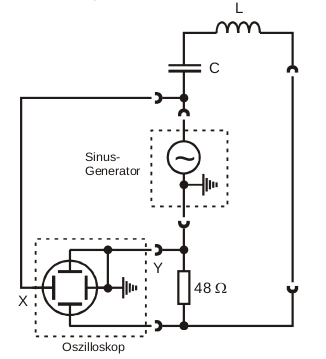
\includegraphics[scale=0.7]{content/Bilder/Test.png}
    \caption{Schaltung zur experimentellen Ermittlung der Resonanzfrequenz.}
    \label{fig:Abb1}
    \end{figure}
    \begin{figure}
        \centering
        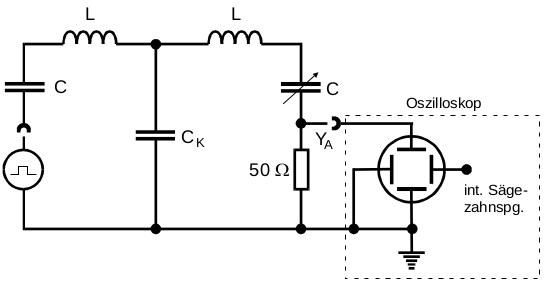
\includegraphics[scale=0.7]{content/Bilder/a_b.png}
        \caption{Schaltung zur experimentellen Ermittlung des Verhältnisses zwischen Schwingungs- und Schwebungsfrequenz.}
        \label{fig:Abb2}
        \end{figure}
\begin{figure}
    \centering
    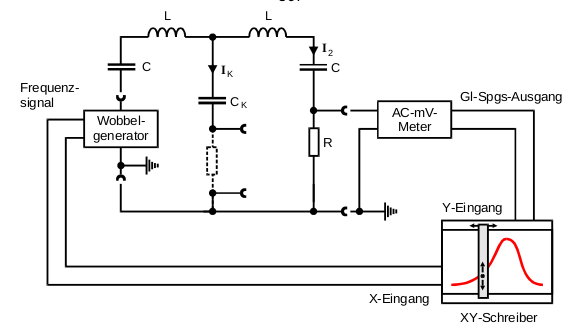
\includegraphics[scale=0.7]{content/Bilder/c.png}
    \caption{Schaltung zur experimentellen Ermittlung des Stroms.}
    \label{fig:Abb3}
    \end{figure}

    \begin{figure}
        \centering
        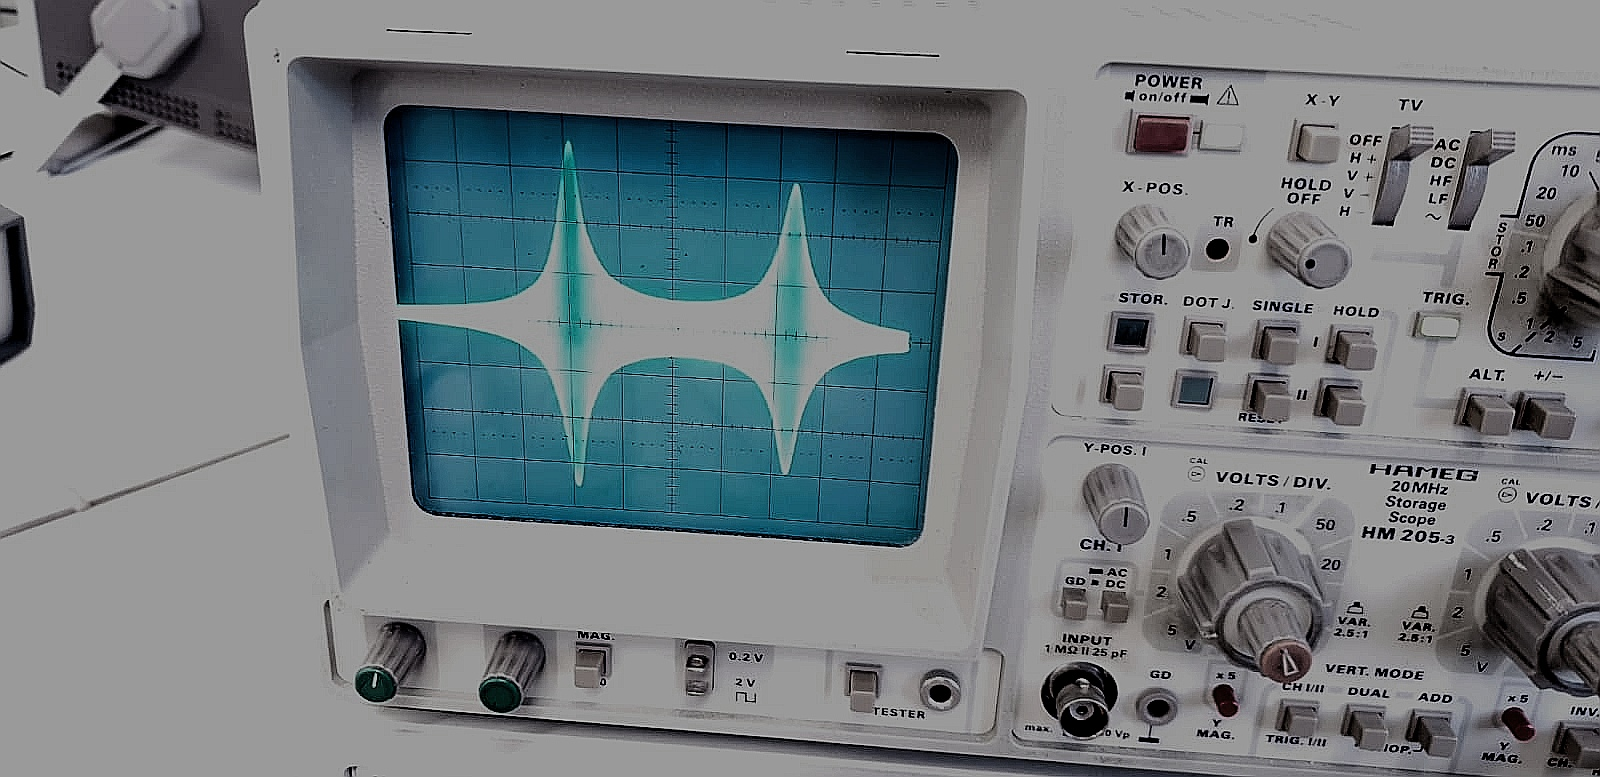
\includegraphics[scale=0.2]{content/Bilder/Titelbild.jpg}
        \caption{Die Spannung im rechten Schwingkreis bei einer sich andauernd wiederholenden sinkenden Frequenz.}
        \label{fig:Abb4}
        \end{figure}
\label{sec:Durchfuehrung}
%Siehe oben? Siehe oben. 